\documentclass{beamer}
\usepackage{animate}
\usepackage{tikz}
\usetheme{metropolis}
\title{Bayesian anomaly detection}
\date{14 November 2023}
\author{Samuel Alan Kossoff Leeney, Will Handley, Dominic Anstey, Eloy de Lera Acedo}
\institute{University of Cambridge}
\begin{document}
  \maketitle
  \section{Bayesian statistics}
  \begin{frame}{Bayes Theorem}
    ``Steve is very shy and withdrawn, invariably helpful but with very little interest in people or in the world of reality. A meek and tidy soul, he has a need for order and structure, and a passion for detail.''
  \end{frame}

  \begin{frame}{Bayes Theorem}
    ``Steve is very shy and withdrawn, invariably helpful but with very little interest in people or in the world of reality. A meek and tidy soul, he has a need for order and structure, and a passion for detail.''

    \begin{itemize}
    \item Is Steve a farmer or a librarian?
    \end{itemize}

  \end{frame}

  \begin{frame}{Bayes Theorem}
    \begin{itemize}
      \item Is Steve a farmer or a librarian?
      \item 90\% of people asked guess librarian~\cite{tversky1986framing}
      \item But there are 20x as many farmers than librarians

    \end{itemize}
    \vfill
    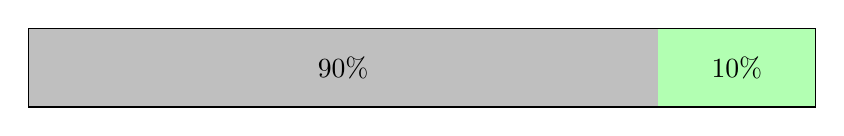
\begin{tikzpicture}
    \fill[gray!50] (0,0) rectangle (8cm,1cm); % 80% filled
    \fill[green!30] (8cm,0) rectangle (10cm,1cm); % remaining 20%
    \draw (0,0) rectangle (10cm,1cm);
    \node at (4cm,0.5cm) {90\%};
    \node at (9cm,0.5cm) {10\%};
    \end{tikzpicture}
  \end{frame}

  \begin{frame}{Bayes Theorem}
    We can approach this problem using Bayes theorem.
    \begin{align}
            \text{likelihood} \times \text{prior} &= \text{posterior} \times \text{evidence} \\
            P(\mathcal{D}|\theta) \times P(\theta) &= P(\theta|\mathcal{D}) \times P(\mathcal{D}), \\
            \mathcal{L} \times \pi &= \mathcal{P} \times \mathcal{Z},
        \end{align}
   \end{frame}

  \section{Anomaly detection}

  \begin{frame}{What do(nt) we look for?}
    \centering
    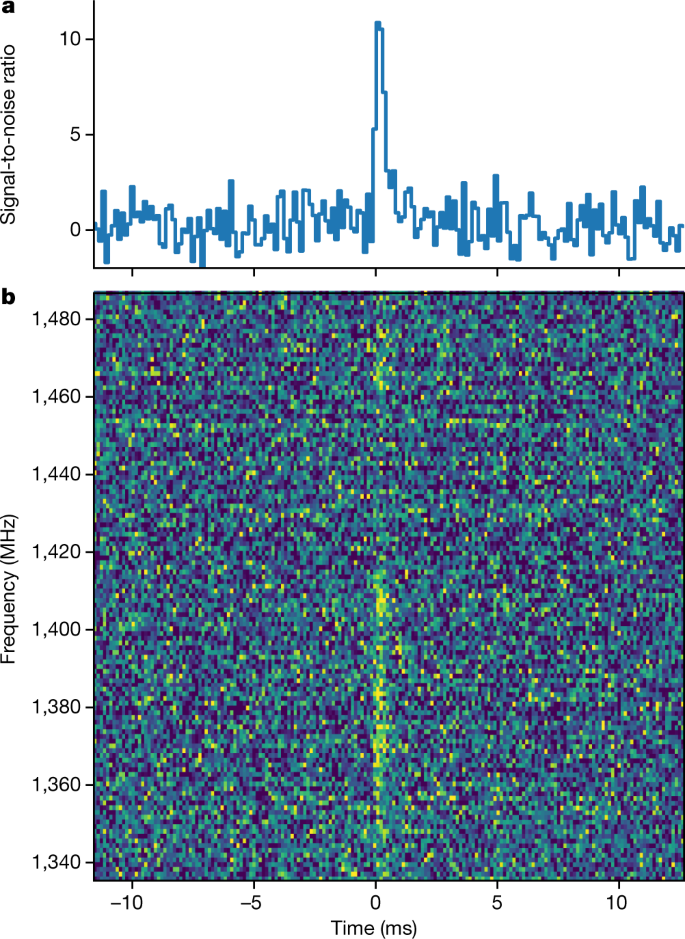
\includegraphics[width=0.8\textwidth]{frb.png}
  \end{frame}

  \begin{frame}{Methodology}
    \footnotesize
    \textbf{a) Generate new likelihood:}
    \begin{equation}
        P(\mathcal{D}_i|\theta) = \begin{cases}
            \mathcal{L}_i(\theta) &: \text{expected}\\
            \Delta^{-1}[ 0<\mathcal{D}_i<\Delta] &: \text{anomalous},
        \end{cases}
    \end{equation}

    \textbf{b) Ascribe Bernoulli prior:}
    \begin{equation}
        P(\varepsilon_i) = p_i^{(1-\varepsilon_i)}(1-p_i)^{\varepsilon_i}.
    \end{equation}

    \textbf{c) Marginalise over epsilon:}
    \begin{equation}
        P(\mathcal{D} | \theta) =\sum_{\varepsilon \in \{ 0, 1 \} ^N}P(\mathcal{D},\varepsilon|\theta)
      \end{equation}


      \textbf{d) Approximate correct mask is most likely}
       \begin{equation}
 P(\mathcal{D}|\theta, \varepsilon_{\mathrm{max}}) \gg \mathrm{max}_j P(\mathcal{D}|\theta,\varepsilon^{(j)})\label{eq:nlo},
\end{equation}

    \textbf{d) Loglikelihood:}
    \begin{equation}
        \log{P(\mathcal{D}|\theta)} = \sum_{i}[{\log{\mathcal{L}_i}+\log({1-p_i})]\varepsilon^{\mathrm{max}}_i + [\log{p}_i - \log{\Delta}](1 - \varepsilon^\mathrm{max}_i})
    \end{equation}
  \end{frame}

    \begin{frame}{Visualising on a simple toy model}
        \begin{columns}
        \column{0.5\textwidth}
        Using numerical sampling techniques to make predictions with $\mathcal{L}$.
        \begin{itemize}
          \item This computes the fraction of posterior believed to `fit` model given the data.
        \end{itemize}
        \column{0.5\textwidth}
        \begin{figure}
            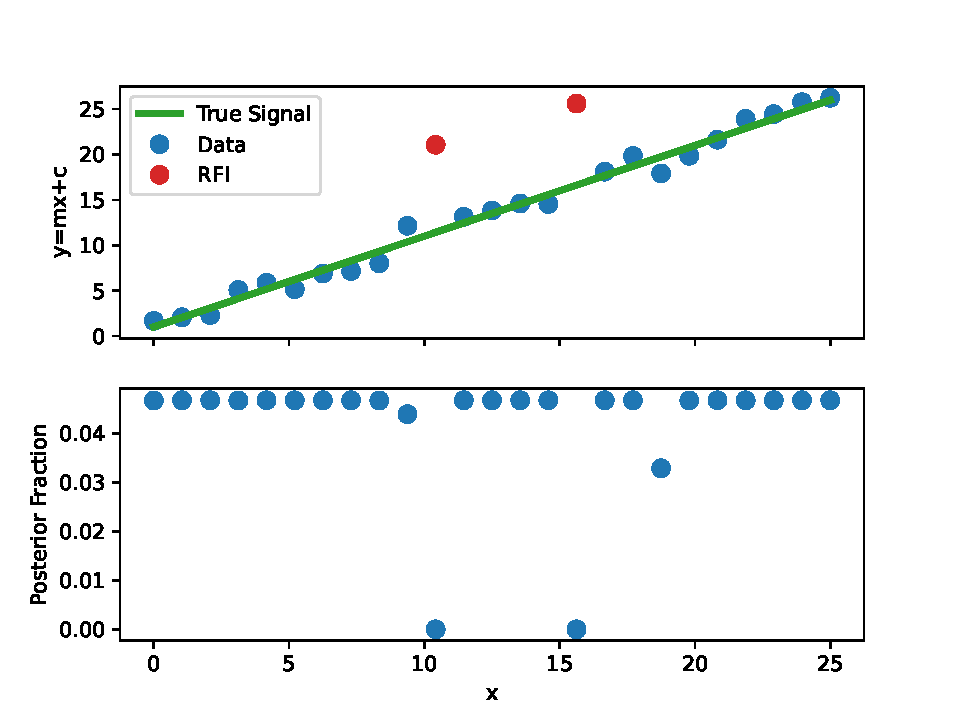
\includegraphics[width=1.1\textwidth]{test.pdf}
        \end{figure}
        \end{columns}
      \end{frame}

    \begin{frame}{Probability thresholding condition $p$}
        \begin{equation}
        \begin{aligned}
        \log{P(\mathcal{D}|\theta)} &= \sum_{i}[{\log{\mathcal{L}_i}+\log({1-p_i})]\varepsilon^{\mathrm{max}} + [\log{p}_i - \log{\Delta}](1 - \varepsilon^\mathrm{max}_i})\label{eq:loglikelihood},
        \end{aligned}
        \end{equation}
        \centering \animategraphics[autoplay, loop, width=11cm]{2}{gif_anest/comb_}{1}{9}
      \end{frame}

      \begin{frame}{Fully automated anomaly detection}
        \begin{itemize}
        \item Putting a prior on $p$, we can fit it dynamically as a free parameter.
        \item This fully automates the anomaly detection process.
        \end{itemize}
    \end{frame}

    \begin{frame}{Initially developed to mitigate for anomalies}
      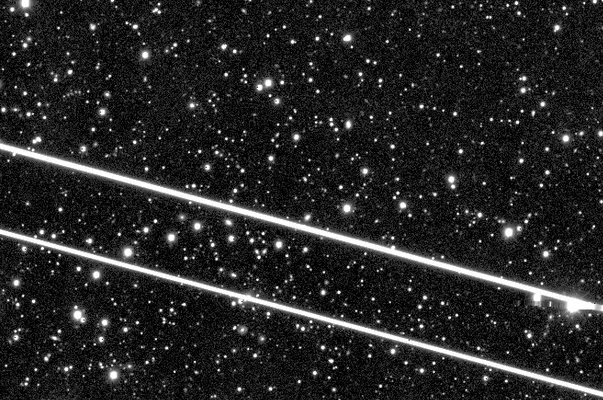
\includegraphics[width=1\textwidth]{starlink2.png}
    \end{frame}

    \begin{frame}{Implement with 2 lines of code}
        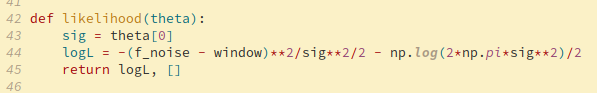
\includegraphics[width=1\textwidth]{logl1.png}
        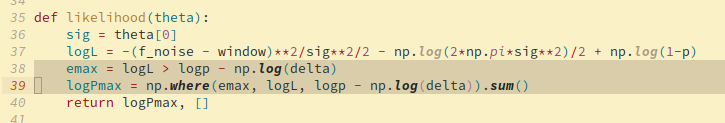
\includegraphics[width=1\textwidth]{logl2.png}
        \centering Tutorial @ github.com/samleeney
    \end{frame}

    \begin{frame}{Read the paper!}
      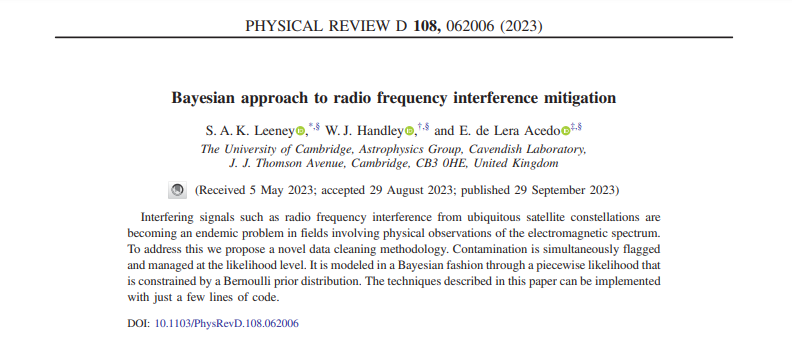
\includegraphics[width=1\textwidth]{paper1.png}
      \href{https://arxiv.org/abs/2211.15448}{arxiv: 2211.15448}
    \end{frame}

    \section{Time sensitive anomaly detection}

    \begin{frame}{Time sensitive likelihood}
        \begin{itemize}
        \item Likelihood from before is extended into two dimensions, becoming
        \end{itemize}
        \begin{multline}\label{eq:time_sep_flagged}
        \log \mathcal{L} \left(\theta\right) = \sum_{ij} \left[\log \mathcal{L}_{ij} \left(\theta\right) + \log\left(1-p_{ij}\right)\right]\epsilon_{ij} +
        \\
        \left[ \log p_{ij} - \log \Delta \right]\left(1-\epsilon_{ij}\right)
        \end{multline}
      \end{frame}


    \begin{frame}{Time sensitive likelihood}
        \begin{itemize}
        \item Computation time of the likelihood grows linearly with the number of time bins used in the data set.
        \end{itemize}
        \begin{multline}\label{eq:time_sep_flagged}
        \log \mathcal{L} \left(\theta\right) = \sum_{ij} \left[\log \mathcal{L}_{ij} \left(\theta\right) + \log\left(1-p_{ij}\right)\right]\epsilon_{ij} +
        \\
        \left[ \log p_{ij} - \log \Delta \right]\left(1-\epsilon_{ij}\right)
        \end{multline}
      \end{frame}

    \begin{frame}
    \frametitle{Speeding up}

    % Start of the two-column layout
    \begin{columns}[T]

        % Left column for bullet points
        \begin{column}{0.5\textwidth}
            \begin{itemize}
                \item Anstey proposes a solution to this problem in~\cite{anstey2023use}.
                \item Common model per time bin is fit jointly.
                \item Speeds up fit but not sensitive to transients.
            \end{itemize}
        \end{column}

        % Right column for screenshots
        \begin{column}{0.5\textwidth}
            \begin{figure}
                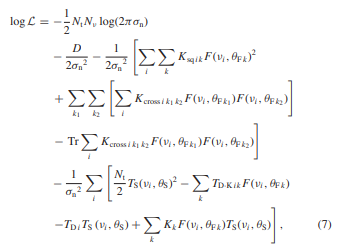
\includegraphics[width=\textwidth]{dom_timedep_math.png}
              \end{figure}
        \end{column}

      \end{columns}
        \begin{tikzpicture}[remember picture, overlay]
        \node [anchor=north east, inner sep=0pt] at ([xshift=-2.5cm, yshift=-1.1cm]current page.north east) {
            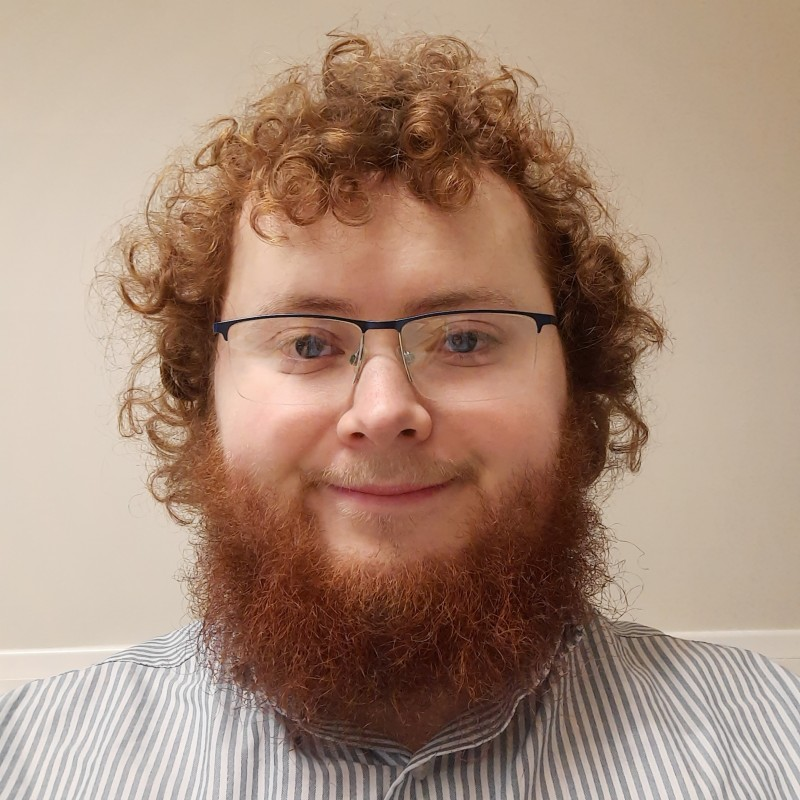
\includegraphics[width=1.7cm]{dom_pic.jpeg} % Adjust the size as needed
        };
        \end{tikzpicture}

      \end{frame}


      \begin{frame}
          \frametitle{Likelihood reweighting}

        \begin{columns}
        \begin{column}{0.5\textwidth}
        \begin{itemize}
          \item Introduced in context of gravitational waves by~\cite{payne2019higher}~\cite{romero2019searching}.
          \item Bayesian sampling techniques spend lots of time at tails of distribution.
          \item Reweighting is essentially a course then fine search, using a simple (fast) then complex (slow) likelihood.
        \end{itemize}
      \end{column}
      \begin{column}{0.5\textwidth}
      \end{column}
        \end{columns}
      \end{frame}

      \begin{frame}
        \frametitle{How does this help us?}
        \begin{columns}
        \begin{column}{0.5\textwidth}
          \begin{itemize}
            \item We can use the fast method for a coarse scan.
            \item Then the slower method for refined scan.
            \item Increases speed massively for larger problems.
        \end{itemize}
      \end{column}
      \begin{column}{0.5\textwidth}
        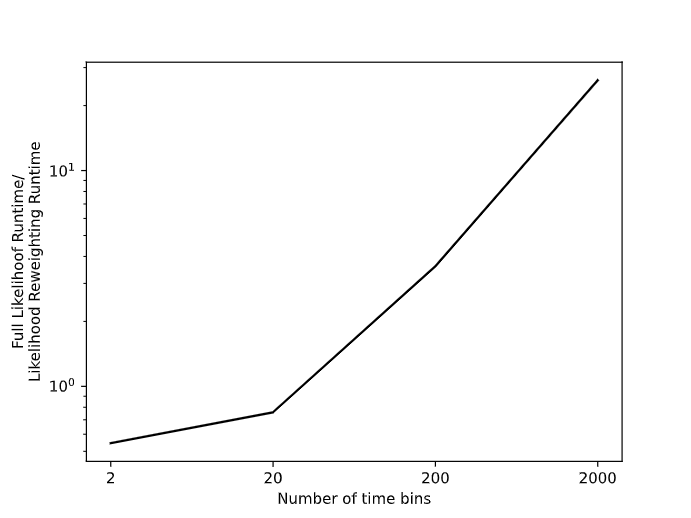
\includegraphics[width=1\textwidth]{lrw_runtime.png}
      \end{column}
    \end{columns}
    \end{frame}

      \begin{frame}
        \frametitle{Testing on a simple toy example}
        \begin{figure}
            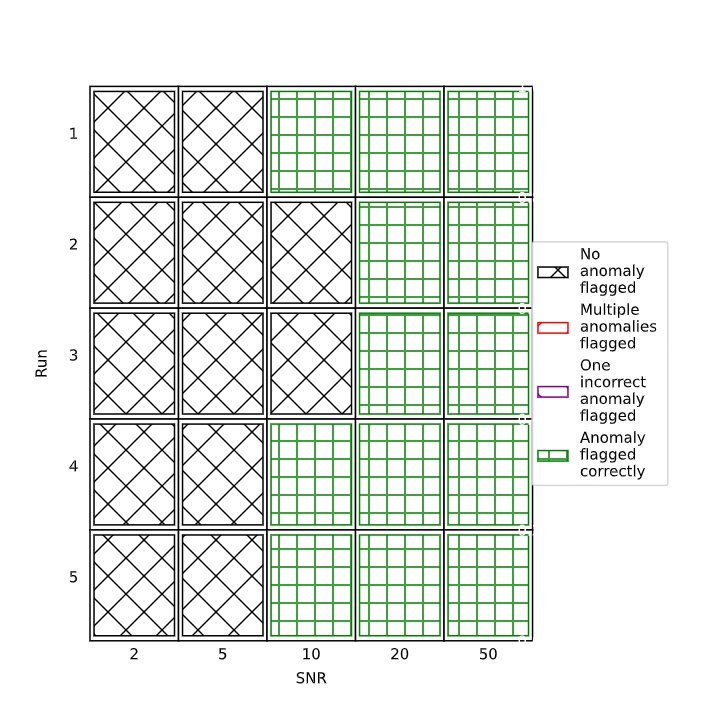
\includegraphics[width=0.7\textwidth]{transient_dom.png}
        \end{figure}
      \end{frame}

      \begin{frame}
        \frametitle{Read the paper!}
        \begin{figure}
        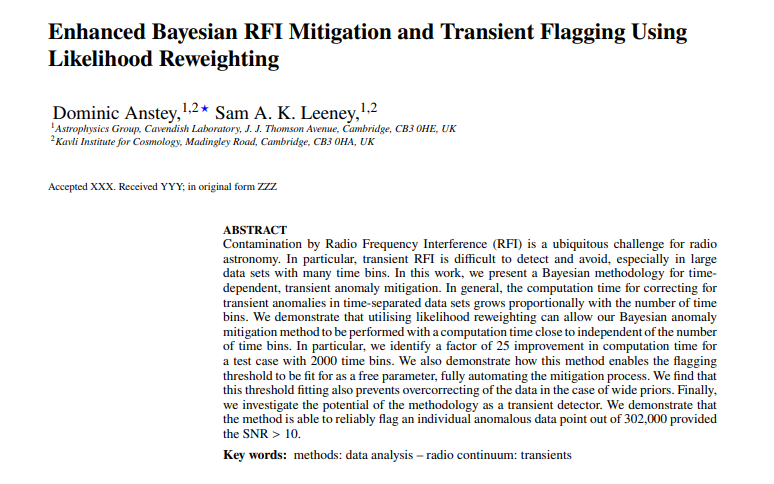
\includegraphics[width=0.7\textwidth]{da_sl_paper.png}
      \end{figure}
      \href{https://arxiv.org/abs/2310.02146}{arxiv: 2310.02146}

      \end{frame}

      \begin{frame}
        \frametitle{Conclusions}
        \begin{columns}
        \begin{column}{0.5\textwidth}
          \begin{itemize}
            \item Fast scans of old data - hopefully find something new!
            \item 2 lines of code to implement into existing Bayesian systems
            \item Colaborate with us!
        \end{itemize}
      \end{column}
      \begin{column}{0.5\textwidth}
        
\includegraphics[width=1\textwidth]{qr.png}
        Scan the QR code for the slides or to contact me!
      \end{column}
    \end{columns}
  \end{frame}

    \begin{frame}[t]{References}
    \bibliographystyle{apalike}
    \bibliography{ref.bib} % if your bibtex file is called example.bib
    \end{frame}

\end{document}
